%
% File: chap05.tex
% Author: Abhushan Sahu
% Description: Introduction chapter where the stuff goes on.
%
\let\textcircled=\pgftextcircled
\chapter{Conclusions and future scope}
\label{chap:intro}

\initial{L}ike all the good things, this too should come to an end.\\
Though it is solely dependent on the University and authorities to actually conclude something out of the report. Still...


%=======

\section{Conclusion}
\label{sec:sec01}

The system has a definitive procedure, that when triggered, it automatically does a few things:

  \begin{description}

\item{$\cdot$ p1} Get Gps position.
\item{$\cdot$ p2} Text Sos number about the position.
\item{$\cdot$ p3} Calls Sos number.
\item{$\cdot$ p4} Sends Gps data to our server.
\item{$\cdot$ p5} Receives all incoming call (till deactivated).
\item{$\cdot$ p6} Play help audio through speakers.

\end{description}

The application system is a unique way to list out a calamity if happens.
It comes very handy for everyone and anyone. \\
The application has a profile management that can be used to specify: 
\clearpage

\begin{figure}


	\centering
	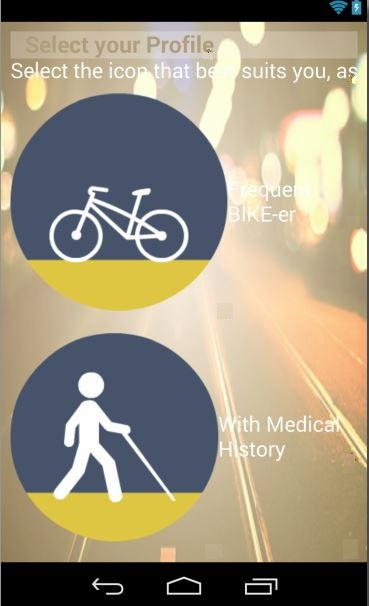
\includegraphics[height=0.35\textheight]{fig01/s_profile}
	\mycaption[Screen-shot of profile selection.]{Screen-shot of profile selection.}
	\label{fig:RHP01}
    

\end{figure}


    \begin{description}
\item{$\cdot$ o1} Riders. \\
Frequent bikers or one who meets the traffic usually are the people of concern here.
\item{$\cdot$ o2} Patients.\\
 That includes people suffering from some sort of mental imbalance, pregnant females, elderly ones.

\end{description}

\subsection{Riders}
\label{subsec:subsec01}

Follows are the data gathered by Government of India, that shows the real face of road safety from ground zero. \\
Note riders are meant by the one that uses vehicle for transportation on a regular basis. Person not suffering from any medical condition should check this one as there profile.


\begin{figure}[h]
	\centering
	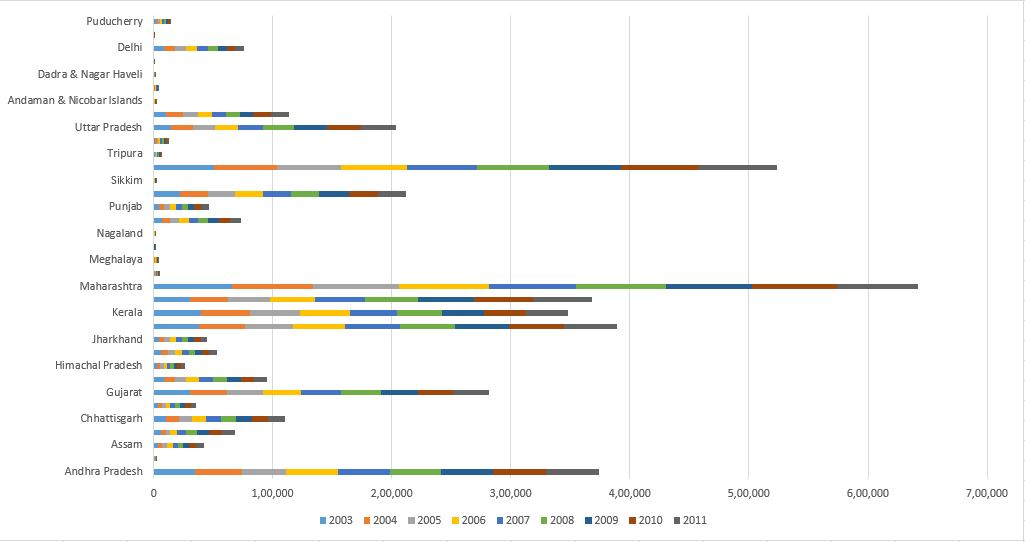
\includegraphics[height=0.35\textheight]{fig01/g_gov_acc}
	\mycaption[Graph of accidents in India.]{Graph of accidents in India in the year 2003-2011.}
	\label{fig:RHP01}
Now this is quite clear that, this is not good.
\end{figure}




\begin{figure}[h]
{	\centering
	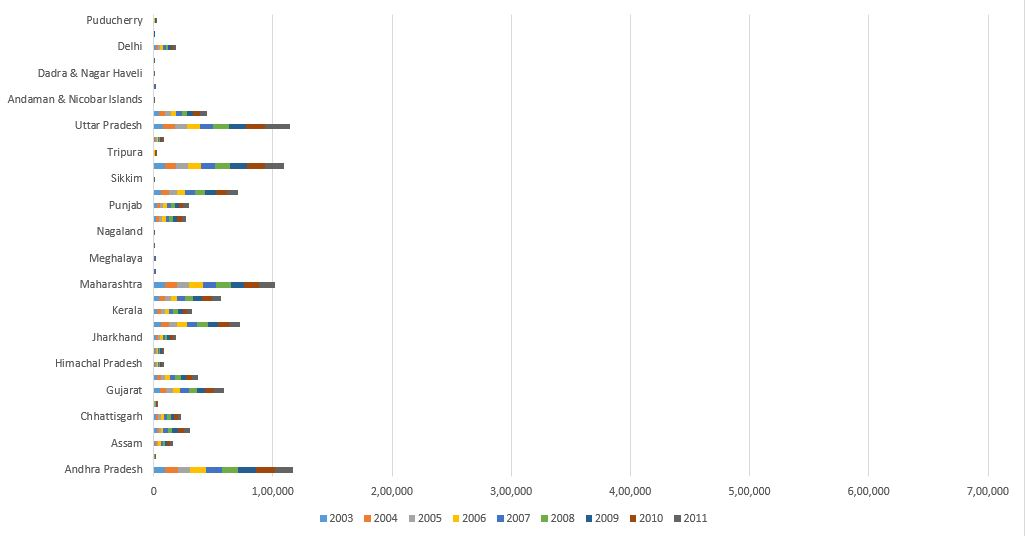
\includegraphics[height=0.35\textheight]{fig01/g_gov_dead}
	\mycaption[Graph of road casualty in India.]{Graph of road casualty in India in the year 2003-2011.}
	\label{fig:RHP01}
}
Now, this graph speaks the bitter/ sad truth. \\
If we happen to apply our application with this, then there is a possibility of 0.24 - 0.6, that the data will get affected. \\
As the hazard can soon be informed of to proper authorities and channels.

\end{figure}

\clearpage

\subsection{Patients}
\label{subsec:subsec02}

Now this column include the category of people that has a certain trait, as listed:
  \begin{description}

\item{$\cdot$ o1} Pregnant Females.
\item{$\cdot$ o2} Parkinson's sufferer.
\item{$\cdot$ o3} People with tangled co-ordination.
\item{$\cdot$ o4} Elderly civilian with knee problem.

\end{description}




\section{Future Scope}
\label{sec:sec02}

The future of this service is bright for the user as-well-as the non-users.
How? It because the filtered data gathered in our servers will be later provided to the government authorities that can list out the potential danger zones in a scope. \\
Also the algorithm used needs a lot of improvement, which we are working on as well. Soon that would be uploaded to git-hub for future development. \\
Also, a provision for user to send the send, and initiate the sos at user's command is under planning. \\
Further, for implementation to global public, there seems to be two options for us:
\begin{description}
\item{$\cdot$ m1} Self marketing and suggesting people to use the application.
\item{$\cdot$ m2} Contacting google, as they have a provision to embed application in their os, as default.
\end{description}

We appreciate your support and enthusiasm for you have read through-out the dissertation. We sure will be glad to hear from you, feel free to mail us at \textit{abhushan@live.com},\textit{ abhinv@gmail.com} for this matter or more.

\newpage\null\thispagestyle{empty}\newpage

